% Weak Scalability Design : Keep Pipeline of Ensembles to show barrier needed in S5 and S6
% Performance, generality with weak scaling (agnostic to kernel)
% Added functionality (do not speak about binding adaptivity to performance or generality)
% In use case: add in why TIES is challenging, and why adaptivity is challenging

\subsection{Experiment Setup}\label{ssec:exp_design}

We perform weak (and strong) scalability experiments on NCSA Blue Waters--a
13.3. petaFLOPS Cray, with 32 Interlago cores/50 GB RAM per node, Cray Gemini,
Lustre shared file system. Our experiments are launched on Blue Waters and
monitored using a persistent virtual machine, as Blue Waters does not allow
for executing applications directly on the login node.


All experiments use HTBAC version 0.1, EnTK version 0.6 and RP version 0.47.
The MD engine used is NAMD-MPI for tasks pertaining to $S1$ - $S4$, while the
analysis stage, $S5$ use AmberTools. For both adaptive and nonadaptive
experiments, the minimization tasks of $S1$ are assigned 100(0) steps, while
the equilibration tasks in $S2$ and $S3$ are assigned 5000 steps. In the
nonadaptive experiments, the production simulation tasks in $S4$ are assigned
50000 steps. For the adaptive experiments, each substage of $S4$ i.e. $S4.1$ -
$S4.4$ is assigned 500,000 steps.

% HTBAC submits a resource request to EnTK, to which EnTK uses RP to acquire
% resources via a single pilot. Accordingly, we request the maximum number of
% cores required by the workload as the number of cores in a pilot. 

We use between 4160 and 33280 cores as indicated in
Figure~\ref{fig:weak_scaling} because the NAMD executable used in all tasks
from $S1$-$S4$ require at least 32 cores per task. From our own scalability
performance measurements of NAMD on Blue Waters, we observe the ideal cores
per task to be 16, however Blue Waters does not permit running multiple MPI
applications on the same node, hence each NAMD task requires a full node to
maintain concurrency.

For the TIES protocol, each pipeline consists of six stages. Each of the simulation
stages contains a task for every unique ($\lambda$, replica) combination.


%EnTK manages the
%queueing of the tasks in accordance with the order and concurrency mandated by
%stages and pipelines. \jhanote{.. need clean separation of implementation
%details from design of experiments}


In the non-adaptive workflow scenario, the first 11 $\lambda$ windows consist
of the following values: $L$ is a vector with
\begin{flalign}
L &= \{ x_i: x_i\in[0,1]\; and\; x_{i+1} = x_i + \delta \}, where\ \delta\ is\ 0.1.
%&$$L=\{ x_i: x_i\in[0,1]\; and\; x_{i+1} = x_i + \delta \}$$%, where $\delta$ is $0.1$.
\end{flalign}

  We append two additional values on both ends of $L$, completing 13 $\lambda$
windows. Each $\lambda$ window consists of five replicas. Therefore there are
a total of 65 tasks for every simulation stage. The production simulations
stage, $s4$ as described in figure~\ref{fig:pst} executes a 4 ns simulation duration. 
The analysis stages of the protocol reduce the number of tasks. 
The first analysis task consists of five tasks where each task performs an 
aggregate analysis over all $\lambda$ windows for each replica. 
The second analysis stage consists of one task that
aggregates the previous results and computes a single average across all
replicas.

%------------------------------------------------------------------------------


\subsection{Scaling and Performance Characterization}

We first characterize the overheads of HTBAC and the runtime system. HTBAC
enables concurrent execution of multiple protocol instances. With each new
protocol instance generated for an application, the HTBAC overhead grows to
match the additional requirement of generating and coordinating protocols.

In order to understand the contribution of the various events in HTBAC, termed
as HTBAC overhead, to the total time to completion (TTC) we construct the
following: $TTC = TTX + T_{O}$ where
 \(TTX\) measures the execution duration across all task, including file
 staging, MD kernel execution, and post-executables, and $T_{O}$ the total
overhead is given by the sum of the constituent overheads: $$T_{O} =
T_{O}\textsuperscript{HTBAC} + T_{O}\textsuperscript{EnTK} +
T_{O}\textsuperscript{RP}$$


%------------------------------------------------------------------------------

\subsubsection{Weak Scaling Experiments}

Here we show weak scalability for the TIES protocol by growing the number of
protocol instances while adhering to the required number of pipelines. By
design of each protocol, an increase in the number of instances simply means
an increase in the number of pipelines. The first weak scalability experiment
demonstrates the behavior of HTBAC, EnTK and RP using the multiple instances
of the TIES protocol. By design of weak scaling, the ratio between the number
of pipelines and cores are kept constant. As the number of cores (measure of
resource) changes by a factor of 2, we introduce twice as many protocol
instances. As designed, the weak scaling property provides insight into the
size of the workload that can be investigated in a given amount of time.

\begin{figure}
  \centering
   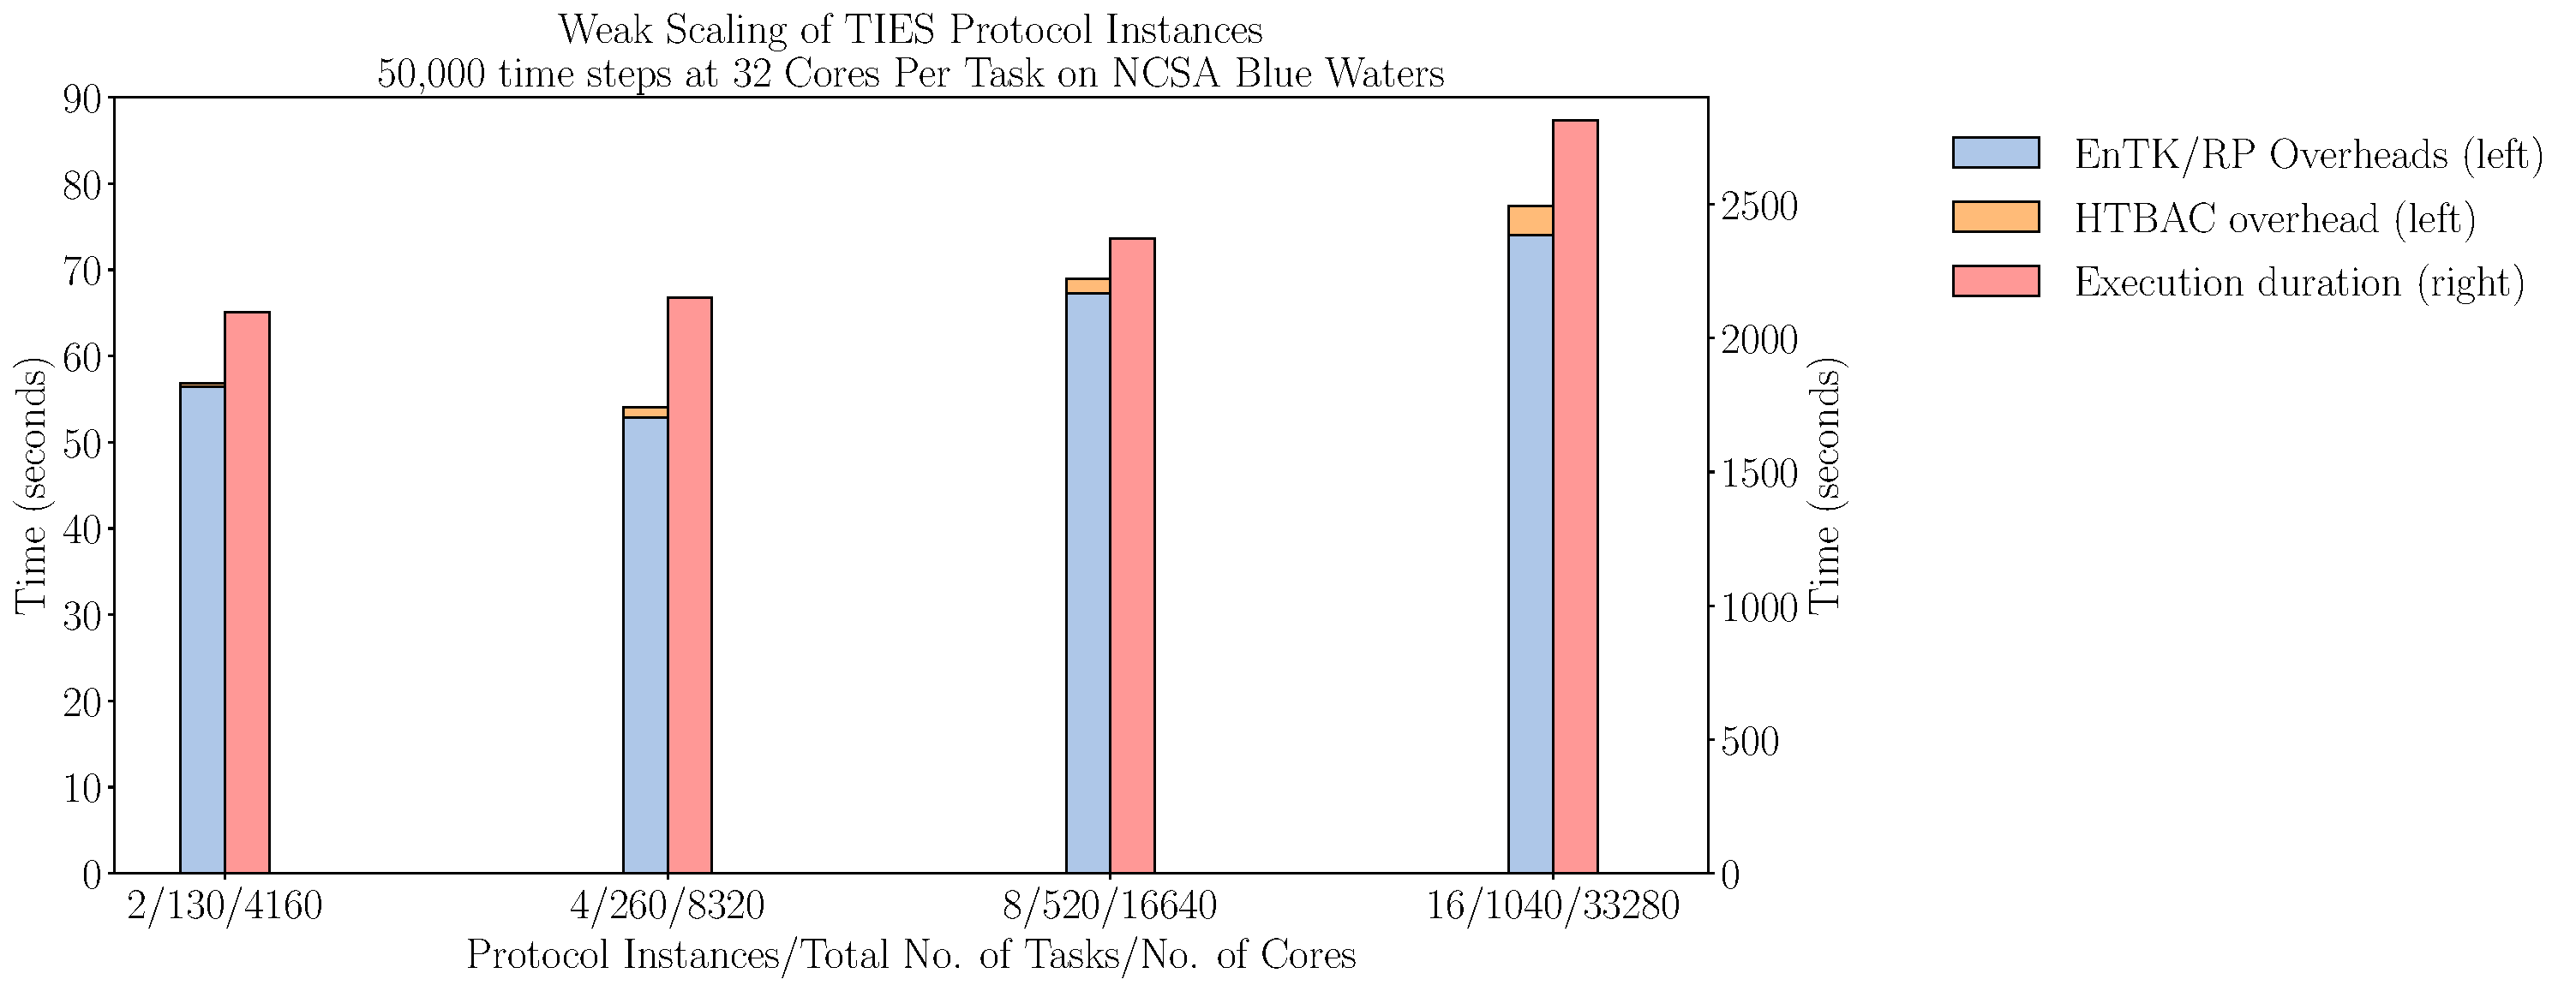
\includegraphics[width=\columnwidth]{./figures/weak_scaling_TIES_instances_50,000_timesteps_with_16_instances.pdf}
  \caption{Weak scaling properties of HTBAC (right side). We investigate the
  weak scaling of HTBAC as the ratio of the number of protocol instances to
  resources is kept constant. (Left) Overheads of HTBAC, and runtime overhead (EnTK/RP) for
  experimental configurations investigating the weak scaling of TIES. We ran two trials for each protocol instance configuration. Error bars in \(TTX\) in 2 and 8-protocol runs are insignficant.}
\label{fig:weak_scaling}
\end{figure}

The HTBAC overhead shows a superlinear increase as we grow the number of protocol 
instances, mainly due to the coordination and generation of additional protocols.
However, the HTBAC overhead is a minimal contributor to \(TTX\). 
The runtime overheads, mainly EnTK and RP, depend on the number of tasks that need to 
be translated in-memory from a Python object to a compute unit (CU) description.
As such, it is expected to grow proportionally to the number of tasks. EnTK
submits CU descriptions to a MongoDB used by RP, and the RP pilot pulls these
descriptions from the same database. This pull operation occurs over a wide
area networks, which introduces varying amounts of latency. In addition, each
stage constructed by EnTK maintains sequential barriers. As such, RP remains
dormant until completion of the current tasks before staging the next tasks.
The impact of the synchronization barriers increases with the number of CUs 
as seen in the 16 protocol instances data point in \ref{fig:weak_scaling}. 

Furthermore, an additional overhead, driven by the aprun launch method, 
increases as we approach a system limit on the number of permissible aprun processes 
when scaling from 8 to 16 protocols, which translates to 520 and 1040 concurrent 
tasks, respectively. We account for the aprun failures in the \(TTX\). Together, 
the EnTK-enabled synchronization barriers and aprun overhead failures introduce 
delays in the scheduling of the CUs and results in higher overheads. Lastly, we notice 
that each additional protocol instance contributes to roughly 55 additional 
seconds in \(TTX\). 



% \subsubsection {Strong Scaling Experiments}

% Next we repeat the same design of the weak scalability experiments but examine
% performance of strong scaling when fixing the number of pipelines and varying
% the resources. The comparison between weak and strong scalability demonstrates
% the overhead introduced by load balancing and scheduling tasks in multiple
% generations.

% (Add in additional points on strong scaling if they come in)

%------------------------------------------------------------------------------


\subsection{Validation Experiment}

HTBAC fully automates the process of calculating the binding affinity of
protein-ligand complexes from reading the input all the way to analyising the
final results. In order to validate the correctness of the results, we have
devised a set of experiments. These experiments are vital to gain confidence
in the algorithm and to prove that it is indeed calculating the correct values.

The validation experiments were based on the original study of Wan et. al.
\cite{Wan2017brd4}. We selected a subset of the protein ligand systems that
were the subject of that study: they are the ligand transformations 3 to 1, 4,
and 7. We then performed a full simulation on all 3 systems and calculated the
binding affinity (see Table~\ref{tab:exp2}) using HTBAC.

The results show that all three $\Delta \Delta$G values are within error bars
of the original study, reinforcing the fact that HTBAC has indeed correctly
implemented the complex workflow of TIES.

\begin{table}
  \centering
  \begin{tabular}{l@{\hskip 1in}r@{\hskip 0.2in}r@{\hskip 0.2in}r}
    \toprule
    System & HTBAC & Wan et. al & Experiment \\
    \midrule
    BRD4 \textbf{3 to 1} & \num{0.39 +- 0.10} &   \num{0.41 +- 0.04} &  \num{0.3 +- 0.09} \\
    BRD4 \textbf{3 to 4} & \num{0.02 +- 0.12} &   \num{0.01 +- 0.06} &  \num{0.0 +- 0.13} \\
    BRD4 \textbf{3 to 7} & \num{-0.88 +- 0.17} &  \num{-0.90 +- 0.08} & \num{-1.3 +- 0.11} \\
    \bottomrule
  \end{tabular}

  \caption{Comparison of the calculated binding free energies using HTBAC, from
  the original study by Wan et. al and experimental data. The two theoretical
  studies used the same protcol in principle. This experiment proved that HTBAC
  has indeed implemented TIES correctly, as the calculated values are either
  the same or within error bar of the original study. All values are in
  \textbf{kcal mol\textsuperscript{-1}}.}
  \label{tab:exp2}


\end{table}

%------------------------------------------------------------------------------

\subsection{Adaptive Experiments}

The TIES workflow can benefit from an adaptive execution environment to improve
the efficiency and accuracy of result. In \emph{adaptive experiments} we
implemented the adapative quadrature algorithm specifically customised for
biosimulations.

In the adaptive workflow, over the course of a protocol instance we alter
the number of $\lambda$ windows being simulated. The position of new $\lambda$
windows depends on the estimated error of the integral measured between
adjacent windows. Increasing the number of $\lambda$ windows in regions of
rapid change will increase the accuracy of the overall integral to a greater
degree than an
arbitrarily placed window. In order to adaptively add lambda windows, we need
access to the $\partial U/\partial\lambda$ values during runtime. Therefore, we break down the
single production simulation stage (S4) from the nonadaptive workflow into
multiple smaller stages, each running for 1 ns. Once each simulation is
complete within a stage a decision is made about whether more $\lambda$ windows
are required, and if so where they should be placed.

We start out the simulation with 5 replicas of \emph{3} equally spaced
$\lambda$ windows, and equilibrate them. 
Then we repeatedly execute 
shorter production simulations followed by an analysis phase which determines where to
place new lambda windows. 
This procedure is repeated until convergence, at which point all
concurrect simulation are terminated. 
We define convergence as the point in
the production-analysis loop at which a desired error threshold is
reached. 

The success of this algorithm is determined by the decision determing 
where additional $\lambda$ windows should be introduced.
In adaptive quadrature, this decision is made by
calculating an error estimate on the integral and comparing this to a threshold value. 
Due to the stochastic nature of biosimulations, it is
non-trivial to determine this error, and as a proof of concept we simplified
this decision to replicate pre-calculated results. In future studies we plan
to replace this with a dynamic decision process.

Inter-node communication introduces a constraint on the number of new lambda windows that can be added at each iteration. 
To reduce the overhead of inter-node communication, simulations must run on an integer number of nodes. This means that the
number of new $\lambda$ windows (i.e. the number of simulations) \emph{has} to be
either doubled or left unchanged. 
If the numer of window is doubled the nodes per simulation can be halved automatically. 
Our prototype algorithm loops through the current $\lambda$ window pairs until this criterion is reached, forcefully adding more if needed.


% I don't think we need this equation here, it's too trivial.
% \begin{flalign}
% L &= \{ x_i: x_i\in[0,1]\; and\; x_{i+1} = x_i + \delta \}, where\ \delta\ is\ 0.5.
% %&$$L=\{ x_i: x_i\in[0,1]\; and\; x_{i+1} = x_i + \delta \}$$%, where $\delta$ is $0.1$.
% \end{flalign}

% For every $\lambda$ window we initialize with five replicas therefore yielding a
% total of 15 tasks. We run 15 tasks for stages $S1$ through $S4.1$. Between
% stages $S4.1$ and $S4.3$ the number of $\lambda$ windows doubles
% for every stage, which doubles the total number of tasks. The last production
% simulation stage, $S4.4$, runs for the remaining 2 ns durations.

\dwwnote{I haven't edited the next sentene as I don't know what it means.}
\jhanote{Any better?}
We introduce only a single degree of freedom relative to baseline ``non-
adaptive" experiments, thus our experiments implement adaptive change in the
lambda window value and not temporal ("when"). HTBAC provides the functional
capability to adaptively deterine the time at which the $\lambda$ window are
determined. However in this paper, we do not investigate the impact of such
adaptivity, as the objective is to determine the feasibility of adaptive
execution and resulting scientific merit of adaptive decision making.



\begin{figure}
  \centering
   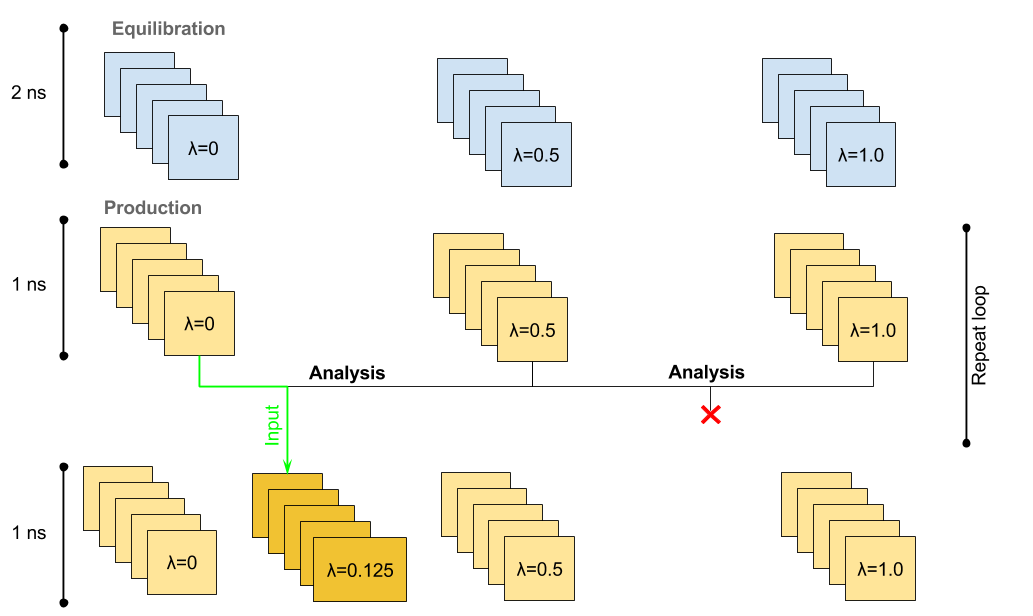
\includegraphics[width=\columnwidth]{figures/Adaptive_TIES_1.png}
  \caption{Illustrating the adaptive workflow. After the 3 inital lambda windows are equilibrated, the first production stage starts. This is followed by analysis at every lambda interval, to decide whether to add a new window in the middle. The production-analysis is repeated for 4 production steps in our implementeation, not shown here.}
\label{fig:adaptive_TIES}
\end{figure}

\subsubsection{Adaptive Quadrature Experiments Results}

One way to visualize the adaptivity in this experiments is to plot the function
and integral approximations at every iteration. Figure~\ref{fig:adapt} shows
how the value of $\Delta$G for one of the test systems improves as the
algorithm places more lambda windowds. It is imporant to note, that the new
points are decided {\it a priori} for reasons discussed above but this is
opaque to the algorithm. This is a proof that we have the adaptive capabilities
and we are paving the way for more advanced biosimulation algorithms.

\begin{figure}
\begin{tikzpicture}
\begin{axis}[
  xlabel=$\lambda$,
  ylabel=$\frac{dU}{d\lambda}$,
  xmin=0,
  xmax=1,
  legend pos=outer north east,
  grid=both,
  ]
  \addplot+[name path=alch_1, mark size=1pt, mark=*, color=blue] table [x=lambda, y=p1v]{figures/alch_1.csv};
  \addlegendentry{Iteration 1: inital lambda spacing};

  \addplot+[name path=alch_2, mark size=1pt, mark=*, color=red] table [x=lambda, y=p1v]{figures/alch_2.csv};
  \addlegendentry{Iteration 2: Increasing number of lambda values};

  \addplot+[name path=alch_3, mark size=1pt, mark=*, color=brown] table [x=lambda, y=p1v]{figures/alch_3.csv};
  \addlegendentry{Iteration 3: Optimial number of lambda values found};

  \addplot+[name path=alch_4, mark size=1pt, mark=*, color=black] table [x=lambda, y=p1v]{figures/alch_4.csv};
  \addlegendentry{Iteration 4: Refining function values at optimial mesh};

  \addplot[name path=line, draw=none] {0};

  \addplot fill between[
    of = alch_1 and line,
    split,
    every even segment/.style = {pattern color=blue!50, pattern=vertical lines},
    every odd segment/.style = {pattern color=blue!50, pattern=vertical lines},
    soft clip={domain=0:1},
  ];

  \addplot fill between[
    of = alch_2 and line,
    split,
    every even segment/.style = {pattern color=red!50, pattern=horizontal lines},
    every odd segment/.style = {pattern color=red!50, pattern=horizontal lines},
    soft clip={domain=0:1},
  ];

  \addplot fill between[
    of = alch_3 and line,
    split,
    every even segment/.style = {pattern color=brown!50, pattern=north east lines},
    every odd segment/.style = {pattern color=brown!50, pattern=north east lines},
    soft clip={domain=0:1},
  ];

\end{axis}
\end{tikzpicture}
\caption{The adaptive algorithm reevaluates the efficiency of the lambda window mesh after every \SI{1}{\nano\second} and makes a decision whether to place more lambda windows inside certain ranges.}
\label{fig:adapt}
\end{figure}



